	\begin{figure}[!h]
	\centering
		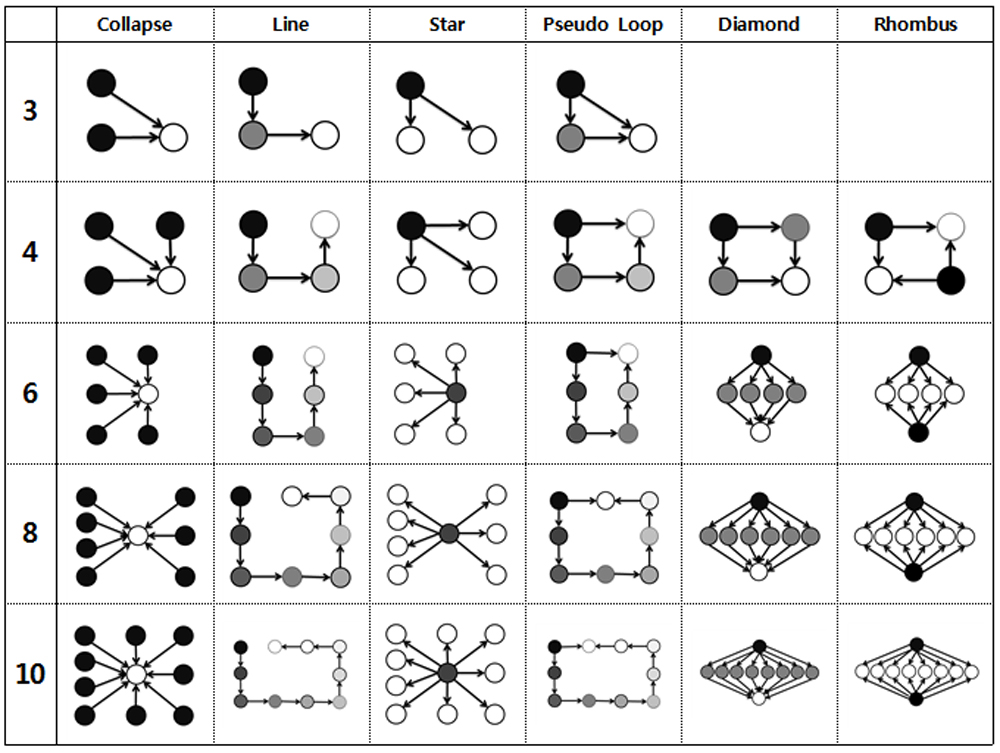
\includegraphics[height=180pt]{Topologies}
		\caption{Bayesian Networks with varying topologies and number of nodes}
	\end{figure}

% 베이지안 네트워크 모형은 노드의 개수가 많아질수록, 그 모형의 어떠한 규칙을 정확히 말하기 어려워진다. 대신 그 모형이 변형됨에도 불구하고 변하지 않는 일정한 성질을 지닌 topology별로 나누어 볼 수 있다. Eitel(2008)은 베이지안 네트워크의 topology를 구분하는 시도를 하였다.
Bayesian network model, as the number of nodes increases, difficult speaking any rules of the model accurately. Instead, even though the model is deformed, topology can be viewed separately separately with a certain properties unchanged. Eitel (2008) was trying to distinguish topology of Bayesian network.

% 여기에서는 이 topology에 따라, 노드 개수를 3, 4, 6, 8, 10개 까지 정하여 모형을 생성한 뒤, 그 모형에 대한 모의 실험을 진행하였다. Cardinality는 2로 제한되었다. 즉 모든 변수는 binary data이다. 확률 값은 $U(0, 1)$의 분포 하에서 임의로 부여하였으며, 우연에 의해 결과가 치우치는 경우를 최소화하기 위해, 모든 실험은 100번 반복한 뒤 그 결과의 합과 표준편차를 계산하였다.
Here, depending on the topology, after creating a set of models of the number of nodes to 3, 4, 6, 8, 10 pieces, we simulate the model. Cardinality was limited to two. In other words, all of the variable is the binary data. The probability value, which is imparted optionally under $ U (0,1) $ distribution. And in order to avoid the influence of chance, all experiments are repeated 100 times, and overall results.